\documentclass[11pt,a4paper]{article}
\usepackage[utf8]{inputenc}
\usepackage[spanish,es-tabla]{babel}
\usepackage[margin=2.5cm]{geometry}
\usepackage{graphicx}
\usepackage{xcolor}
\usepackage{fancyhdr}
\usepackage{titlesec}
\usepackage{booktabs}
\usepackage[most]{tcolorbox}
\usepackage{hyperref}
\usepackage{float}
\usepackage{amsmath}

% Definición de Colores Corporativos
\definecolor{CafePrimary}{HTML}{7C4A3A}     % Café oscuro
\definecolor{CafeSecondary}{HTML}{5D4037}   % Café medio
\definecolor{CafeAccent}{HTML}{4CAF50}      % Verde WhatsApp / Éxito
\definecolor{DarkTitle}{HTML}{3E2723}      % Título oscuro
\definecolor{LightBg}{HTML}{FDFBF7}        % Fondo beige muy claro
\definecolor{BorderColor}{HTML}{D7CCC8}    % Color de bordes suaves
\definecolor{TextMuted}{HTML}{757575}      % Texto atenuado

% Configuración de Hyperref
\hypersetup{
    colorlinks=true,
    linkcolor=CafePrimary,
    filecolor=CafeSecondary,      
    urlcolor=CafeAccent,
    pdftitle={Manual de Usuario - Café Pa'l Monte Gestión},
    pdfpagemode=FullScreen,
}

% Fuentes sans-serif para un look moderno de manual de usuario
\usepackage{helvet}
\renewcommand{\familydefault}{\sfdefault}

% Configuración de Títulos de Sección
\titleformat{\section}
  {\color{CafePrimary}\normalfont\Large\bfseries}
  {\thesection}{1em}{}
\titleformat{\subsection}
  {\color{CafeSecondary}\normalfont\large\bfseries}
  {\thesubsection}{1em}{}
\titleformat{\subsubsection}
  {\color{DarkTitle}\normalfont\normalsize\bfseries}
  {\thesubsubsection}{1em}{}

% Configuración de Encabezados y Pies de Página
\pagestyle{fancy}
\fancyhf{}
\fancyhead[L]{\textcolor{CafeSecondary}{\small\leftmark}}
\fancyhead[R]{\textcolor{CafeSecondary}{\small\thepage}}
\fancyfoot[L]{\textcolor{CafeSecondary}{\small Café Pa'l Monte Gestión · v1.0.0}}
\fancyfoot[R]{\textcolor{CafeSecondary}{\small Pontificia Universidad Javeriana Cali}}
\renewcommand{\headrulewidth}{0.4pt}
\renewcommand{\footrulewidth}{0.4pt}
\addtolength{\headheight}{3pt}

% Configuración de Cajas de Mensaje (tcolorbox)
\newtcolorbox{notaBox}[1][]{
  colback=blue!5!white,
  colframe=blue!50!black,
  fonttitle=\bfseries,
  title=Nota Importante,
  arc=2mm,
  #1
}
\newtcolorbox{advertenciaBox}[1][]{
  colback=red!5!white,
  colframe=red!60!black,
  fonttitle=\bfseries,
  title=Advertencia,
  arc=2mm,
  #1
}
\newtcolorbox{consejoBox}[1][]{
  colback=green!5!white,
  colframe=green!60!black,
  fonttitle=\bfseries,
  title=Consejo de Uso,
  arc=2mm,
  #1
}

\begin{document}

% ==========================================
% PORTADA
% ==========================================
\begin{titlepage}
    \centering
    \vspace*{1.5cm}
    
    {\Huge\bfseries\color{CafePrimary} Café Pa'l Monte Gestión}\\[0.5cm]
    {\Large\bfseries\color{CafeSecondary} Sistema de Sincronización y Gestión de Pedidos}\\[0.2cm]
    {\large\color{CafeSecondary} WhatsApp Business Web}\\[1.5cm]
    
    
\includegraphics[width=0.32\textwidth]{app.png}\\[2cm]
    
    {\large\bfseries\color{DarkTitle} MANUAL DE USUARIO FINAL}\\[0.5cm]
    {\large Versión de Producción · Estable}\\[1.5cm]
    
    \vfill
    
    \begin{tcolorbox}[colback=LightBg,colframe=CafeSecondary,arc=2mm,halign=center]
        \textbf{Autores:}\\
        Brayan Zuluaga \quad Jhon Mejias \quad Juan Collazos \quad Joshua Mendez\\
        \vspace{0.2cm}
        \textbf{Pontificia Universidad Javeriana Cali}\\
        Facultad de Ingeniería y Ciencias \\
        Mayo, 2026
    \end{tcolorbox}
\end{titlepage}

\newpage

% ==========================================
% TABLA DE CONTENIDO
% ==========================================
\tableofcontents
\newpage

% ==========================================
% INTRODUCCIÓN
% ==========================================
\section{Introducción}
El crecimiento y la digitalización de los negocios de comercio local han transformado la forma en que los productores interactúan con sus clientes. \textbf{Café Pa'l Monte Gestión} nace como una solución integral a la necesidad de gestionar y consolidar los pedidos generados de manera cotidiana a través del canal de \textbf{WhatsApp Business Web}.

En los entornos comerciales dinámicos, el flujo de pedidos a través de WhatsApp puede volverse abrumador, propenso a errores humanos (omisiones, registros duplicados, estados desactualizados) y difícil de analizar financieramente a largo plazo. Esta aplicación de escritorio está específicamente diseñada para actuar como un puente seguro y local entre su cuenta comercial de WhatsApp y una base de datos local robusta.

\subsection{Propósito del Documento}
Este manual tiene como objetivo guiar al usuario final en el manejo de la interfaz del software, abarcando desde la instalación básica y la vinculación segura de su cuenta de WhatsApp, hasta el análisis detallado de ventas y la exportación de reportes administrativos. Este documento está exento de tecnicismos de desarrollo y se enfoca puramente en la operación comercial y la resolución de problemas cotidianos de la aplicación.

\subsection{Características Clave del Sistema}
\begin{itemize}
    \item \textbf{Sincronización Inteligente:} Extrae de manera segura y automática la información de cada orden desde el menú oficial de pedidos de WhatsApp Business Web.
    \item \textbf{Prevención Activa de Duplicados:} Cada pedido cuenta con un identificador único (ID de WhatsApp), lo que previene la redundancia de datos incluso si el sistema realiza múltiples pasadas de sincronización.
    \item \textbf{Gestión y Control Local:} Almacena toda la información de forma local y privada (SQLite). Los datos del negocio no son compartidos con servidores externos, garantizando privacidad absoluta.
    \item \textbf{Dashboard Financiero (Panel):} Muestra indicadores clave de rendimiento (KPIs) como facturación neta, total de órdenes y distribución por estados en tiempo real.
    \item \textbf{Módulo de Analítica Avanzado:} Genera gráficos automáticos de la operación para facilitar la toma de decisiones financieras (ventas anuales, mensuales, productos más vendidos, etc.).
    \item \textbf{Exportación de Reportes:} Genera con un solo clic informes en formato \textbf{PDF} listos para imprimir y hojas de cálculo \textbf{Excel} detalladas para su posterior procesamiento contable.
\end{itemize}

\newpage

% ==========================================
% REQUISITOS E INSTALACIÓN
% ==========================================
\section{Requisitos del Sistema e Instalación}

Para asegurar un funcionamiento óptimo y fluido de la aplicación, el equipo de cómputo debe cumplir con ciertas condiciones básicas. A continuación, se detallan los requisitos del sistema y el proceso de puesta en marcha.

\subsection{Requisitos del Sistema}
\begin{itemize}
    \item \textbf{Sistema Operativo:} Windows 10 o Windows 11 de 64 bits.
    \item \textbf{Navegador Internet:} Google Chrome o Microsoft Edge (se recomienda tenerlos actualizados a su última versión estable).
    \item \textbf{Conexión a Red:} Conexión estable a Internet tanto en la computadora como en el teléfono celular que contiene la cuenta principal de WhatsApp Business.
    \item \textbf{Resolución de Pantalla:} Mínimo 1024 $\times$ 768 píxeles.
\end{itemize}

\subsection{Proceso de Instalación para el Usuario}
El sistema se distribuye de manera compacta para evitar instalaciones complejas o configuraciones de registros del sistema operativo:

\begin{enumerate}
    \item \textbf{Localizar el archivo comprimido:} Identifique el archivo comprimido con el nombre \textbf{``CafePalMonte''} (formato ZIP o similar) entregado por el equipo técnico.
    \item \textbf{Descomprimir el contenido:} Haga clic derecho sobre el archivo comprimido y seleccione la opción \textbf{``Extraer todo...''} o \textbf{``Extraer aquí''}. Se recomienda extraer los archivos en una carpeta de fácil acceso, como su directorio de documentos o el escritorio de Windows.
    \item \textbf{Ubicación de archivos:} Una vez descomprimido, se abrirá una carpeta llamada \textbf{CafePalMonte}. Dentro de ella encontrará los siguientes elementos clave:
    \begin{itemize}
        \item \textbf{CafePalMonte.exe:} Este es el archivo ejecutable principal de la aplicación. Al hacer doble clic en él, la aplicación se iniciará de inmediato.
        \item \textbf{Carpeta \_internal:} Esta carpeta almacena los archivos lógicos y las librerías necesarias para el funcionamiento interno de la aplicación.
    \end{itemize}
\end{enumerate}

\begin{advertenciaBox}
No modifique, renombre, mueva ni elimine la carpeta \textbf{\_internal} ni ninguno de los archivos contenidos en su interior. Hacerlo provocará que la aplicación deje de funcionar de inmediato y requerirá volver a extraer el paquete original.
\end{advertenciaBox}

\newpage

% ==========================================
% PRIMEROS PASOS Y VINCULACIÓN
% ==========================================
\section{Primeros Pasos: Conexión con WhatsApp Business}

Al ejecutar la aplicación por primera vez, el sistema se iniciará en modo desconectado. Es necesario vincular su cuenta comercial de WhatsApp mediante un código QR para permitir que el sistema lea la información de los pedidos.

\subsection{Iniciar Conexión}
Para comenzar con el proceso de conexión, siga los pasos descritos a continuación:

\begin{enumerate}
    \item Abra la aplicación haciendo doble clic sobre el archivo \textbf{CafePalMonte.exe}.
    \item Diríjase al panel lateral izquierdo (de color café oscuro) y localice el botón verde \textbf{``Conectar WhatsApp''} en la sección de conexión inferior.
\end{enumerate}

\begin{figure}[H]
    \centering
    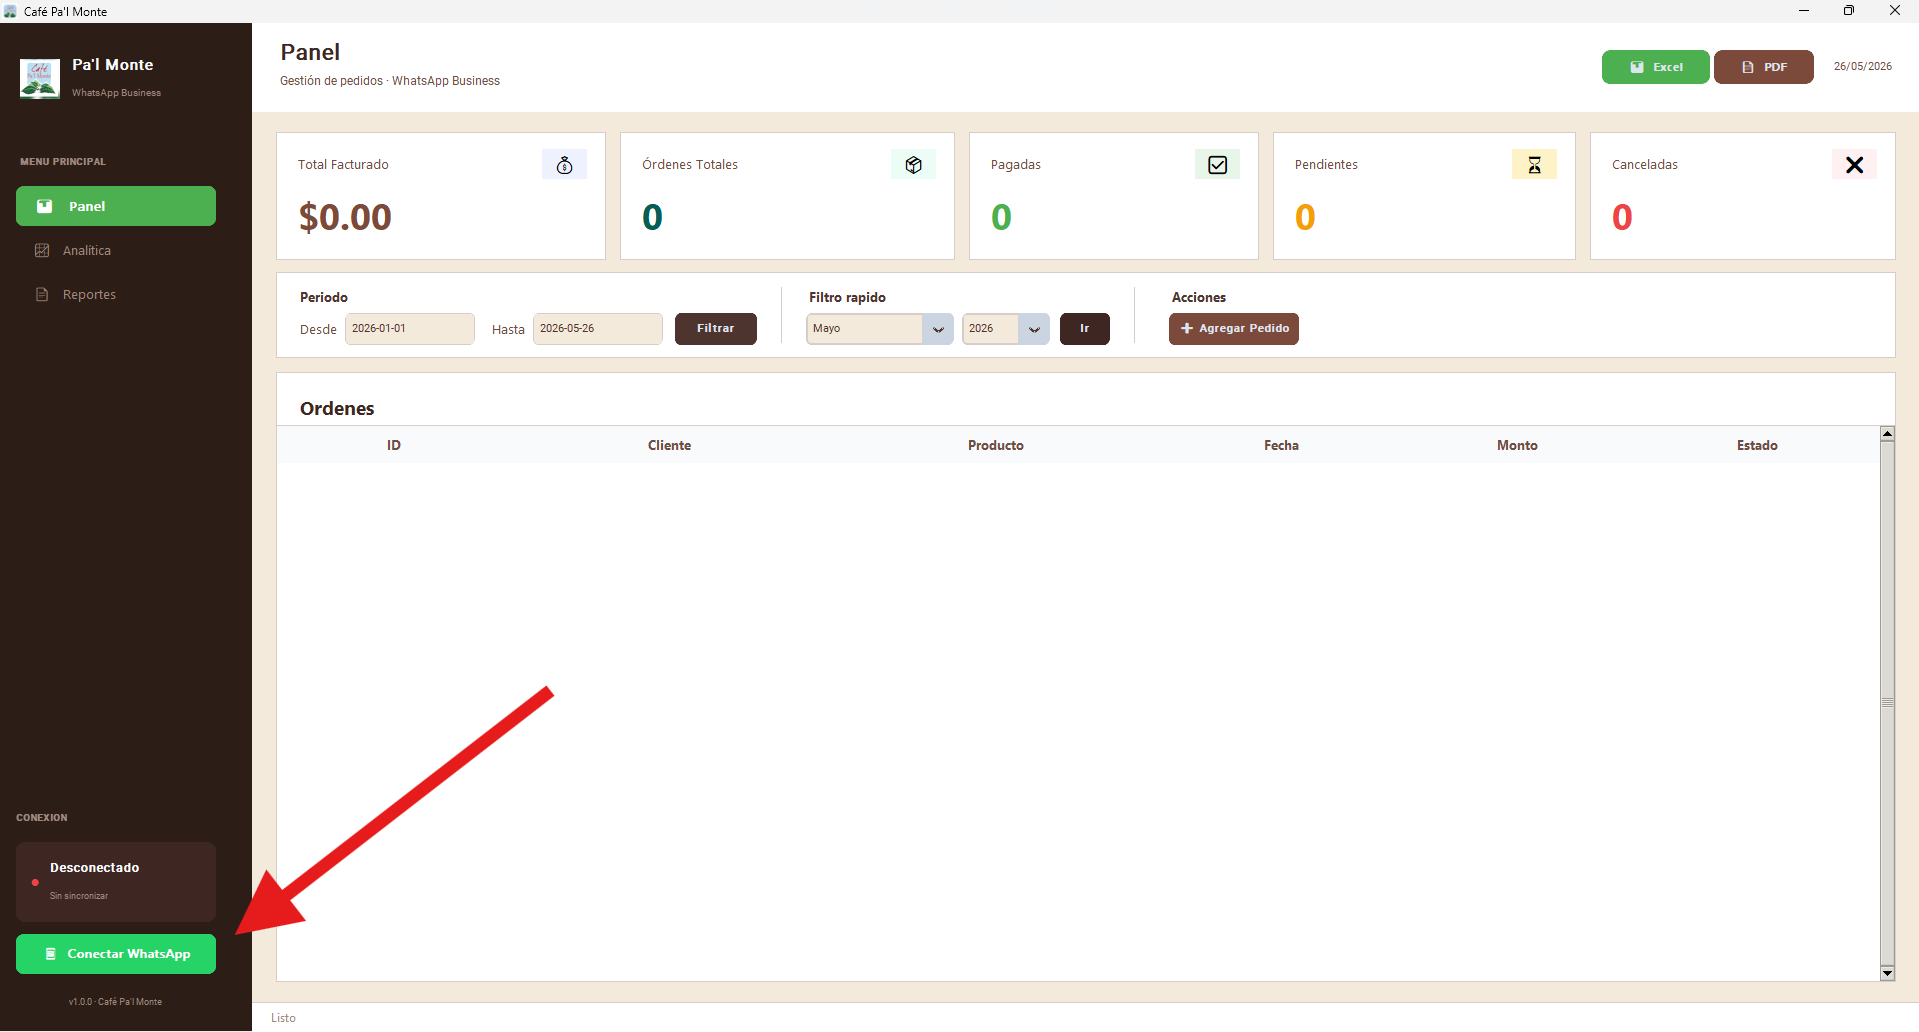
\includegraphics[width=0.7\textwidth]{image1.png}
    \caption{Ubicación del botón Conectar WhatsApp en el panel lateral izquierdo.}
    \label{fig:conectar_wsp}
\end{figure}

\subsection{Escaneo del Código QR}
Al hacer clic en el botón \textbf{``Conectar WhatsApp''}, el sistema abrirá de manera automática una ventana de navegación controlada que cargará la pantalla oficial de vinculación de \textbf{WhatsApp Web}.

\begin{figure}[H]
    \centering
    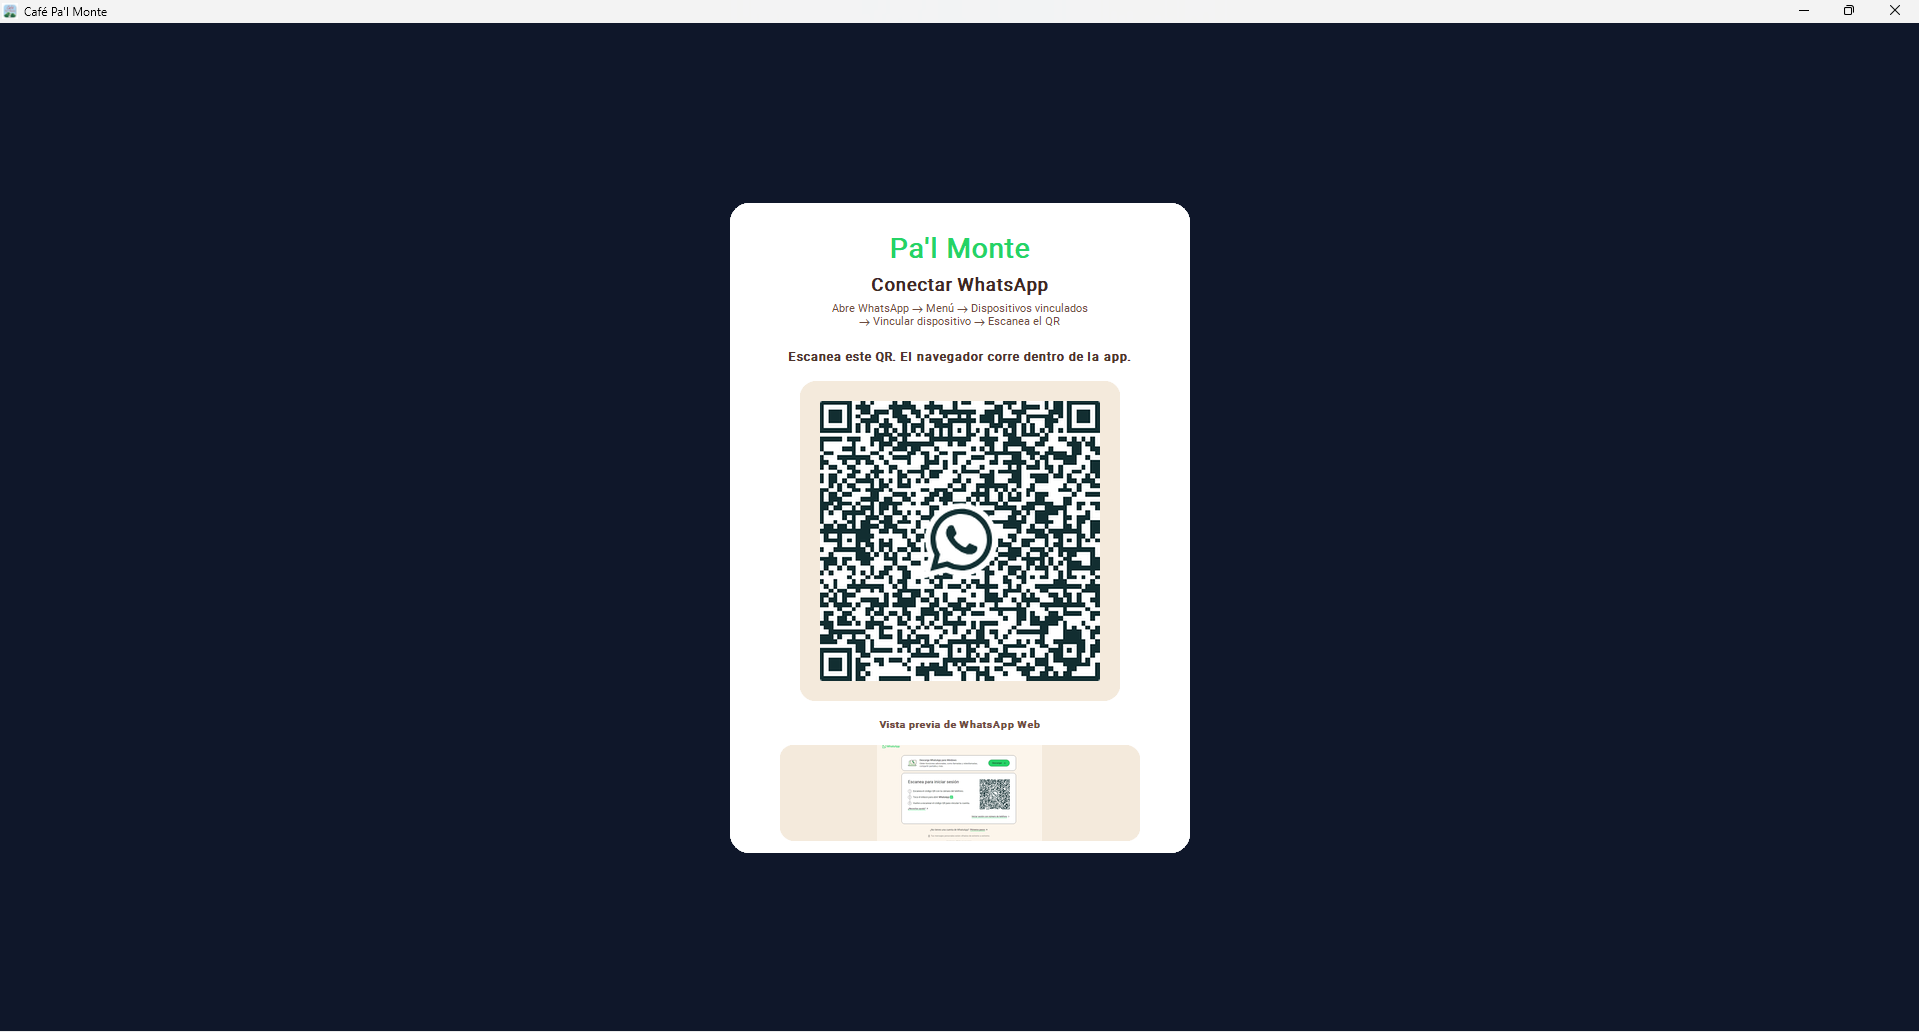
\includegraphics[width=0.8\textwidth]{image2.png}
    \caption{Ventana controlada que muestra el código QR de vinculación.}
    \label{fig:qr_code}
\end{figure}

Para vincular su dispositivo:
\begin{enumerate}
    \item Tome su teléfono móvil (el cual debe tener activa la cuenta de WhatsApp Business asociada a su negocio).
    \item En la aplicación de WhatsApp de su teléfono celular, acceda al menú de configuración (icono de tres puntos en Android o el engranaje de Configuración en iPhone).
    \item Seleccione la opción \textbf{``Dispositivos vinculados''}.
    \item Presione el botón \textbf{``Vincular un dispositivo''}.
    \item Use la cámara de su celular para escanear el código QR que se proyecta en la pantalla de la computadora.
    \item Mantenga la ventana abierta y su teléfono conectado hasta que la vinculación se complete. Al finalizar, la ventana del navegador mostrará sus chats habituales y el panel lateral del programa cambiará de estado.
\end{enumerate}

\subsection{Estado de Conexión y Control de Sincronización}
Una vez establecida la conexión con éxito, la interfaz de la aplicación cambiará para reflejar el estado activo. En el panel izquierdo se mostrará un indicador circular de color verde junto al texto \textbf{``Conectado''} y la hora de la última sincronización.

\begin{figure}[H]
    \centering
    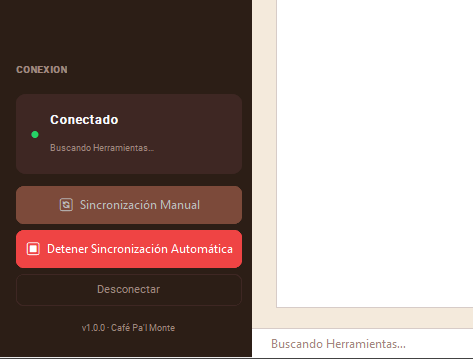
\includegraphics[width=0.7\textwidth]{image3.png}
    \caption{Panel lateral en estado Conectado con opciones avanzadas de sincronización.}
    \label{fig:connected_status}
\end{figure}

El sistema ofrece tres botones principales de interacción de sincronización en este estado:

\begin{itemize}
    \item \textbf{Sincronización Automática:} Este es el modo operativo estándar. Mientras la aplicación se mantenga abierta y conectada, el sistema buscará periódicamente nuevas órdenes registradas en WhatsApp Web en segundo plano sin interrumpir su trabajo.
    \item \textbf{Sincronización Manual:} Si acaba de recibir un pedido urgente y desea verlo reflejado de inmediato en el Panel sin esperar la rutina automática, haga clic en este botón para realizar una lectura instantánea de los pedidos activos en la sesión de WhatsApp.
    \item \textbf{Desconectar / Cerrar Sesión:} Cierra la sesión activa en el navegador controlado y desconecta el sistema.
\end{itemize}

\begin{advertenciaBox}
Use la opción de \textbf{Desconectar} o cerrar sesión con precaución. Al hacerlo, el navegador controlado cerrará la sesión de WhatsApp Business. Aunque las órdenes ya guardadas no se perderán de su base de datos local del software, al volver a conectar deberá escanear nuevamente el código QR. Se recomienda no cerrar la sesión diariamente, sino dejarla vinculada y cerrar la aplicación normalmente. Se sugiere desvincular o refrescar la sesión una vez por semana para mantener una carga óptima y segura del sistema.
\end{advertenciaBox}

\newpage

% ==========================================
% PANEL DE GESTIÓN (DASHBOARD)
% ==========================================
\section{Módulo de Gestión de Pedidos (Panel)}

El \textbf{Panel} (o Dashboard) es la pantalla de inicio por defecto de la aplicación. Su objetivo es brindar una visión general de la actividad comercial diaria y permitir la administración directa de los pedidos registrados en el sistema.

\begin{figure}[H]
    \centering
    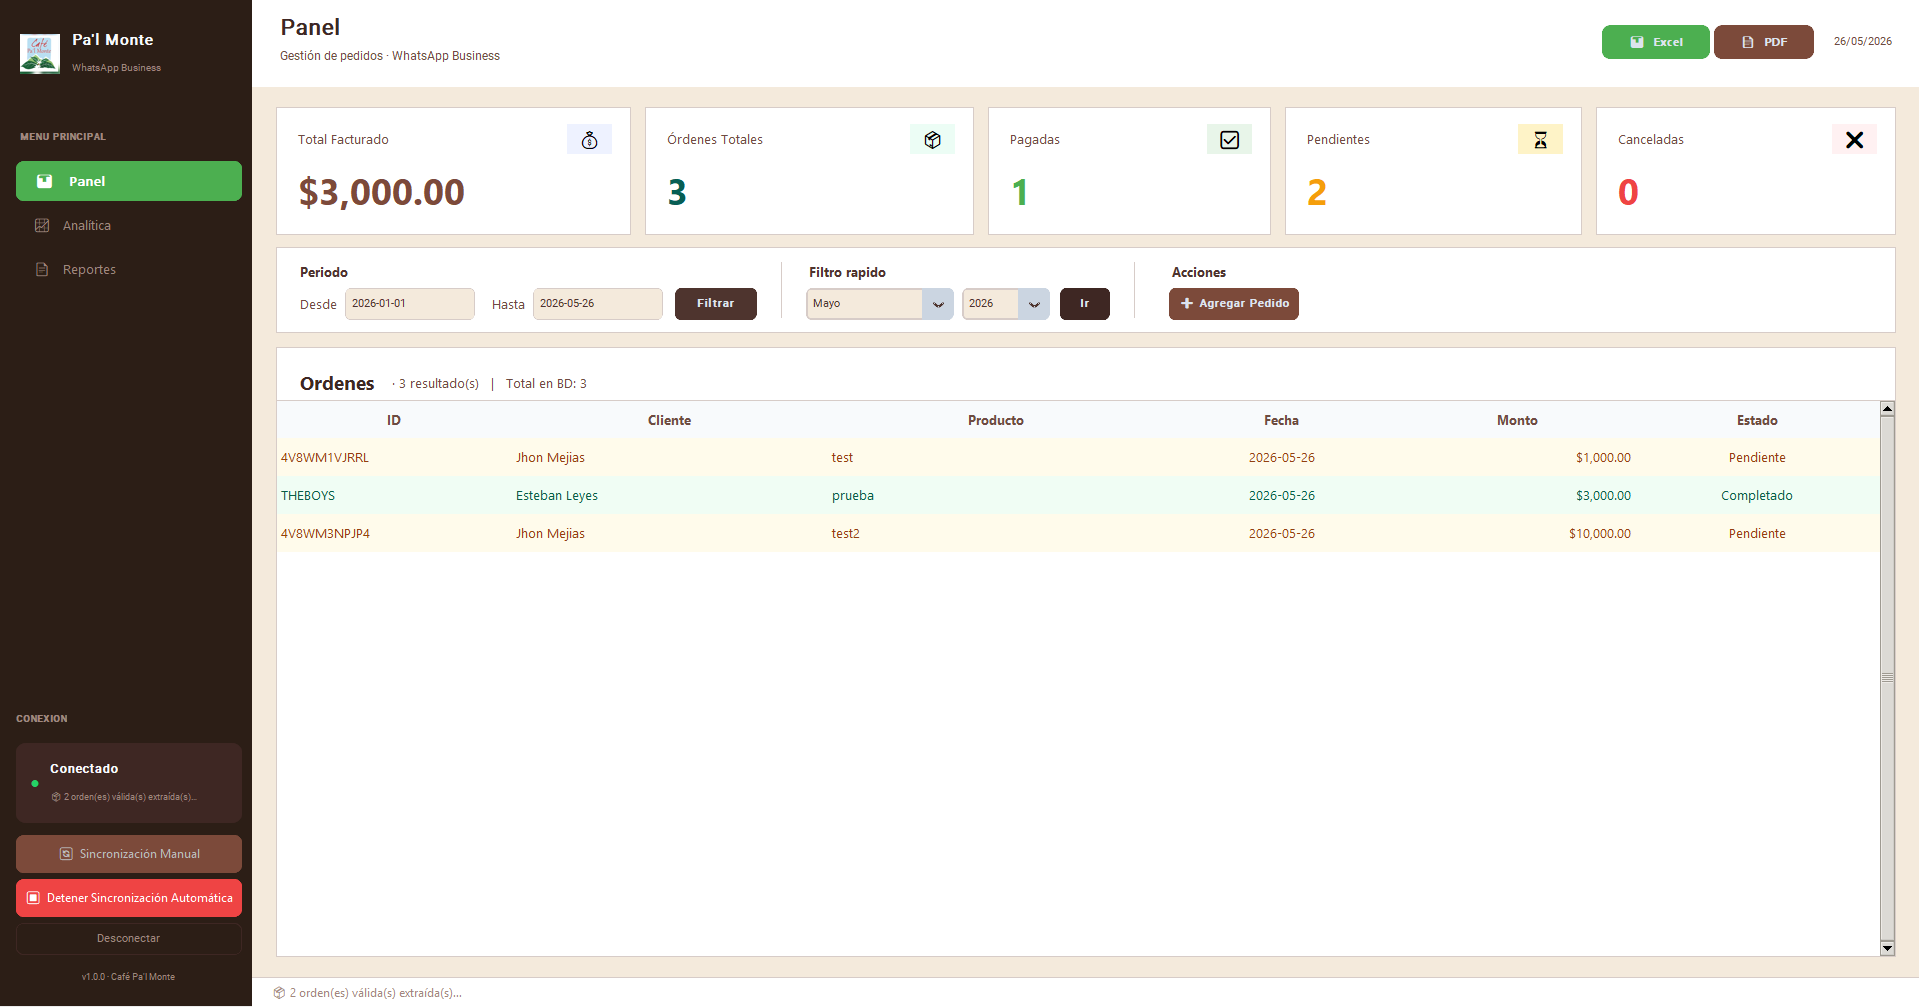
\includegraphics[width=0.9\textwidth]{image4.png}
    \caption{Vista general del Módulo de Panel.}
    \label{fig:panel_overview}
\end{figure}

\subsection{Indicadores de Rendimiento (KPIs)}
En la parte superior del panel se encuentran cinco tarjetas de indicadores clave que resumen la información financiera y operativa del periodo de consulta activo:

\begin{enumerate}
    \item \textbf{Total Facturado (icono de bolsa de dinero):} Suma monetaria neta del valor de las órdenes cobradas. \textit{Consulte la subsección~\ref{subsec:paid_states} para conocer qué estados aportan a este monto.}
    \item \textbf{Órdenes Totales (icono de caja):} Cantidad absoluta de pedidos registrados en el sistema durante el periodo consultado.
    \item \textbf{Pagadas (icono de marca de verificación verde):} Cantidad de pedidos que se encuentran en estado ``Completado'' o ``Entregado''.
    \item \textbf{Pendientes (icono de reloj de arena):} Pedidos que han sido creados pero cuyo pago o entrega aún está por definirse.
    \item \textbf{Canceladas (icono de equis roja):} Cantidad de transacciones anuladas.
\end{enumerate}

\subsection{Estados de Pago e Ingreso}\label{subsec:paid_states}
Para efectos administrativos, es fundamental comprender qué estados de orden influyen en el cálculo del \textbf{Total Facturado}. 
\begin{itemize}
    \item \textbf{Estados Aprobatorios (Generan ingreso):} Completado, Enviado, Envío en preparación y Entregado. Todos los pedidos bajo estas etiquetas se suman en la métrica del Total Facturado.
    \item \textbf{Estados No Aprobatorios (No generan ingreso):} Pendiente (pago solicitado o pendiente de validación) y Cancelado (anulado). Estos pedidos se visualizan en la lista general y alteran sus respectivas métricas, pero su monto monetario se excluye de la sumatoria de ingresos netos.
\end{itemize}

\subsection{Filtros de Fecha y Búsqueda}
Abajo de los KPIs se sitúa la barra de filtrado temporal. Permite delimitar las órdenes que se visualizan en la tabla inferior y que se toman en cuenta para los cálculos rápidos:

\begin{figure}[H]
    \centering
    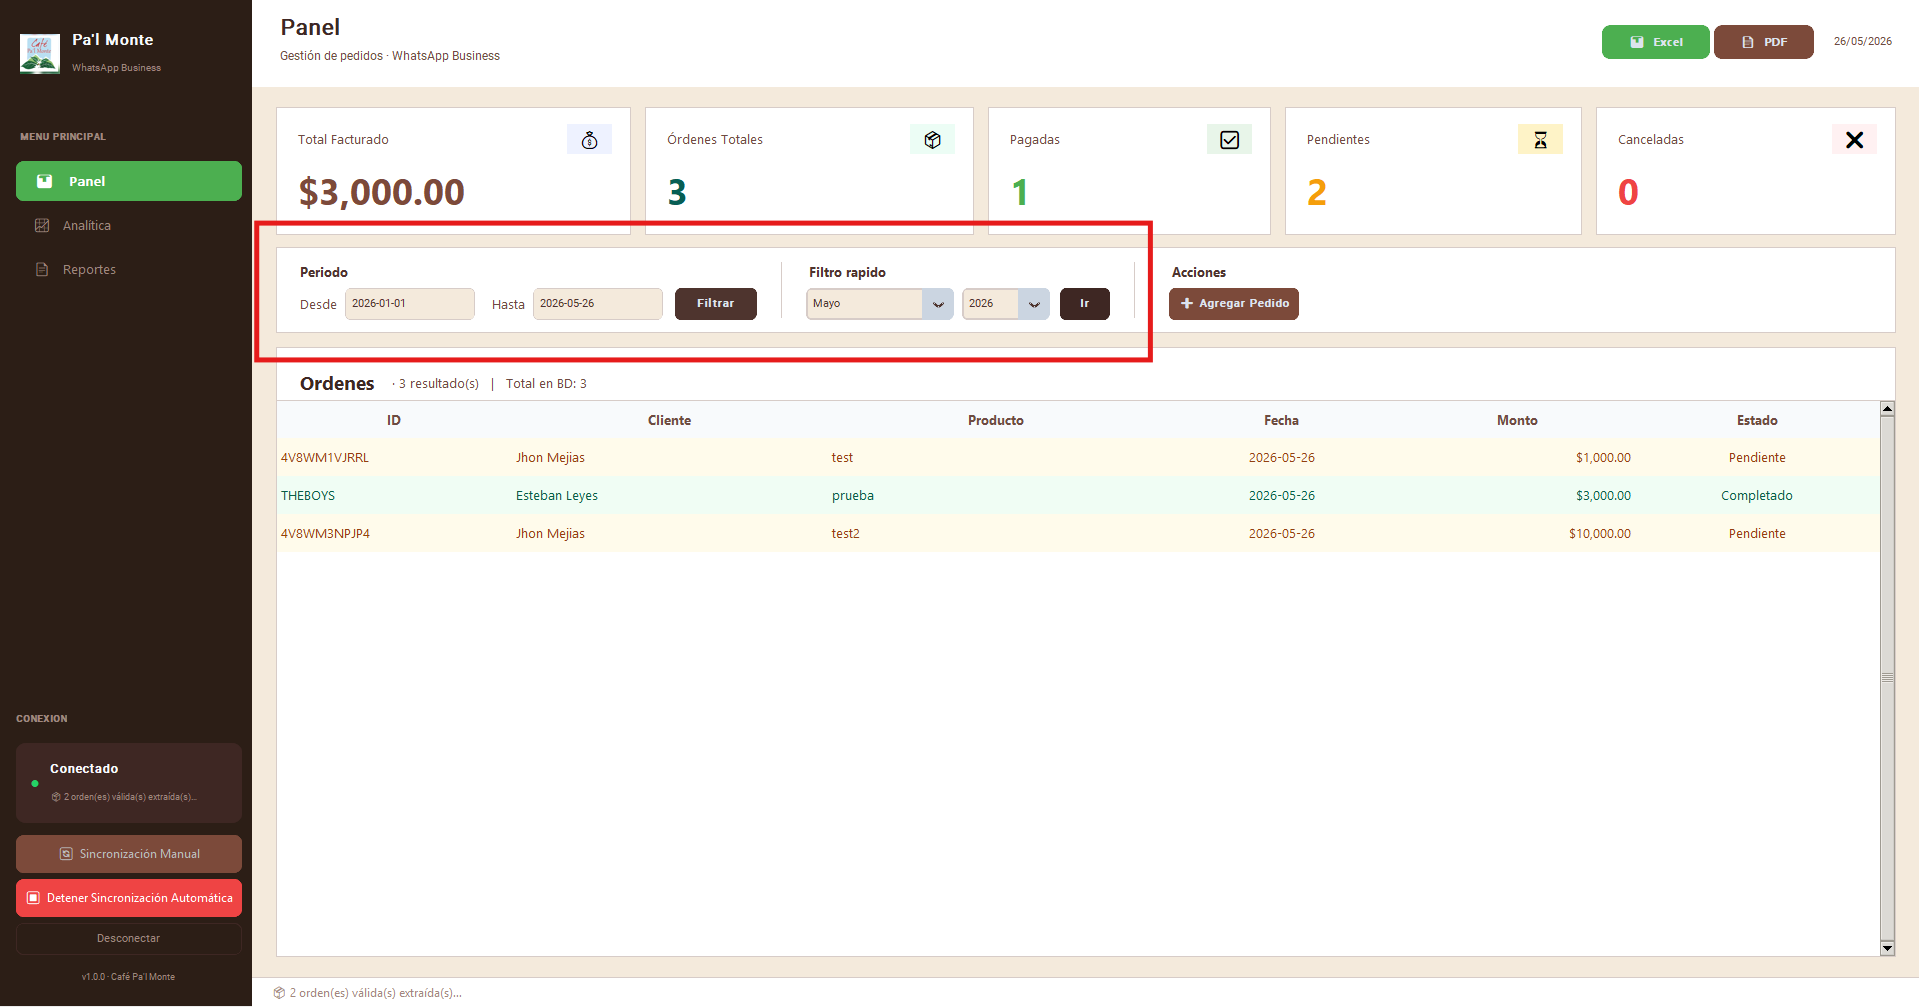
\includegraphics[width=0.9\textwidth]{image5.png}
    \caption{Barra de filtros de fechas personalizada y opción rápida mensual.}
    \label{fig:filters}
\end{figure}

\begin{itemize}
    \item \textbf{Filtrado por Rango de Fechas:} Utilice los campos \textbf{``Desde''} y \textbf{``Hasta''} para definir un rango personalizado. Al hacer clic en cualquiera de estos campos, se desplegará un calendario interactivo que le permitirá seleccionar la fecha deseada. Al finalizar, haga clic en \textbf{``Filtrar''}.
    \item \textbf{Filtro Rápido Mensual:} Ubicado al lado derecho del rango. Seleccione un mes específico del menú desplegable y un año de la lista contigua, y haga clic en \textbf{``Ir''} para ajustar la tabla a ese periodo de facturación exacto de forma veloz.
\end{itemize}

\subsection{Agregar Pedido de Forma Manual}
En ocasiones, por diversas razones operativas (compras presenciales, llamadas telefónicas directas o pedidos que no alcanzaron a sincronizarse debido a un cierre abrupto de la sesión de WhatsApp), es necesario registrar un pedido de forma manual.

\begin{figure}[H]
    \centering
    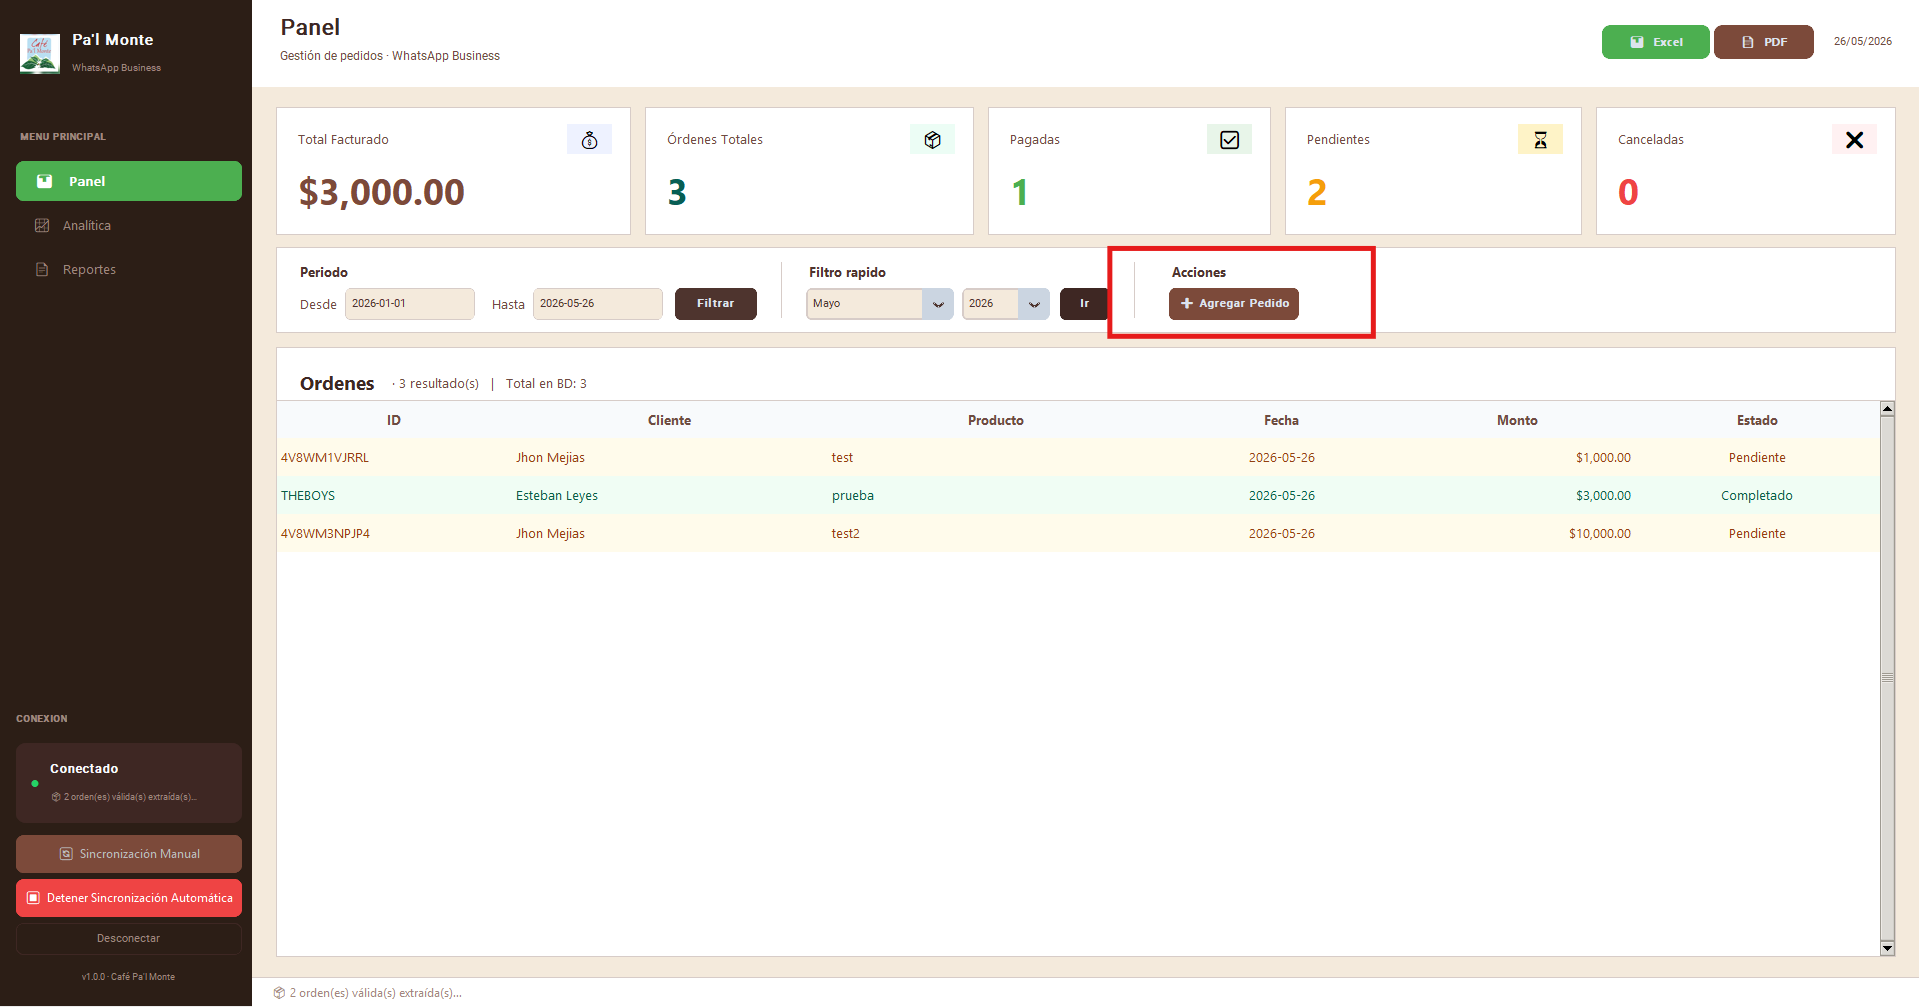
\includegraphics[width=0.9\textwidth]{image6.png}
    \caption{Ubicación de la acción para agregar pedidos de forma manual.}
    \label{fig:add_button}
\end{figure}

Para registrar un pedido de forma manual:
\begin{enumerate}
    \item Haga clic en el botón café \textbf{``+ Agregar Pedido''} ubicado en la barra de filtros.
    \item Se abrirá una ventana emergente con un formulario en blanco.
\end{enumerate}

\begin{figure}[H]
    \centering
    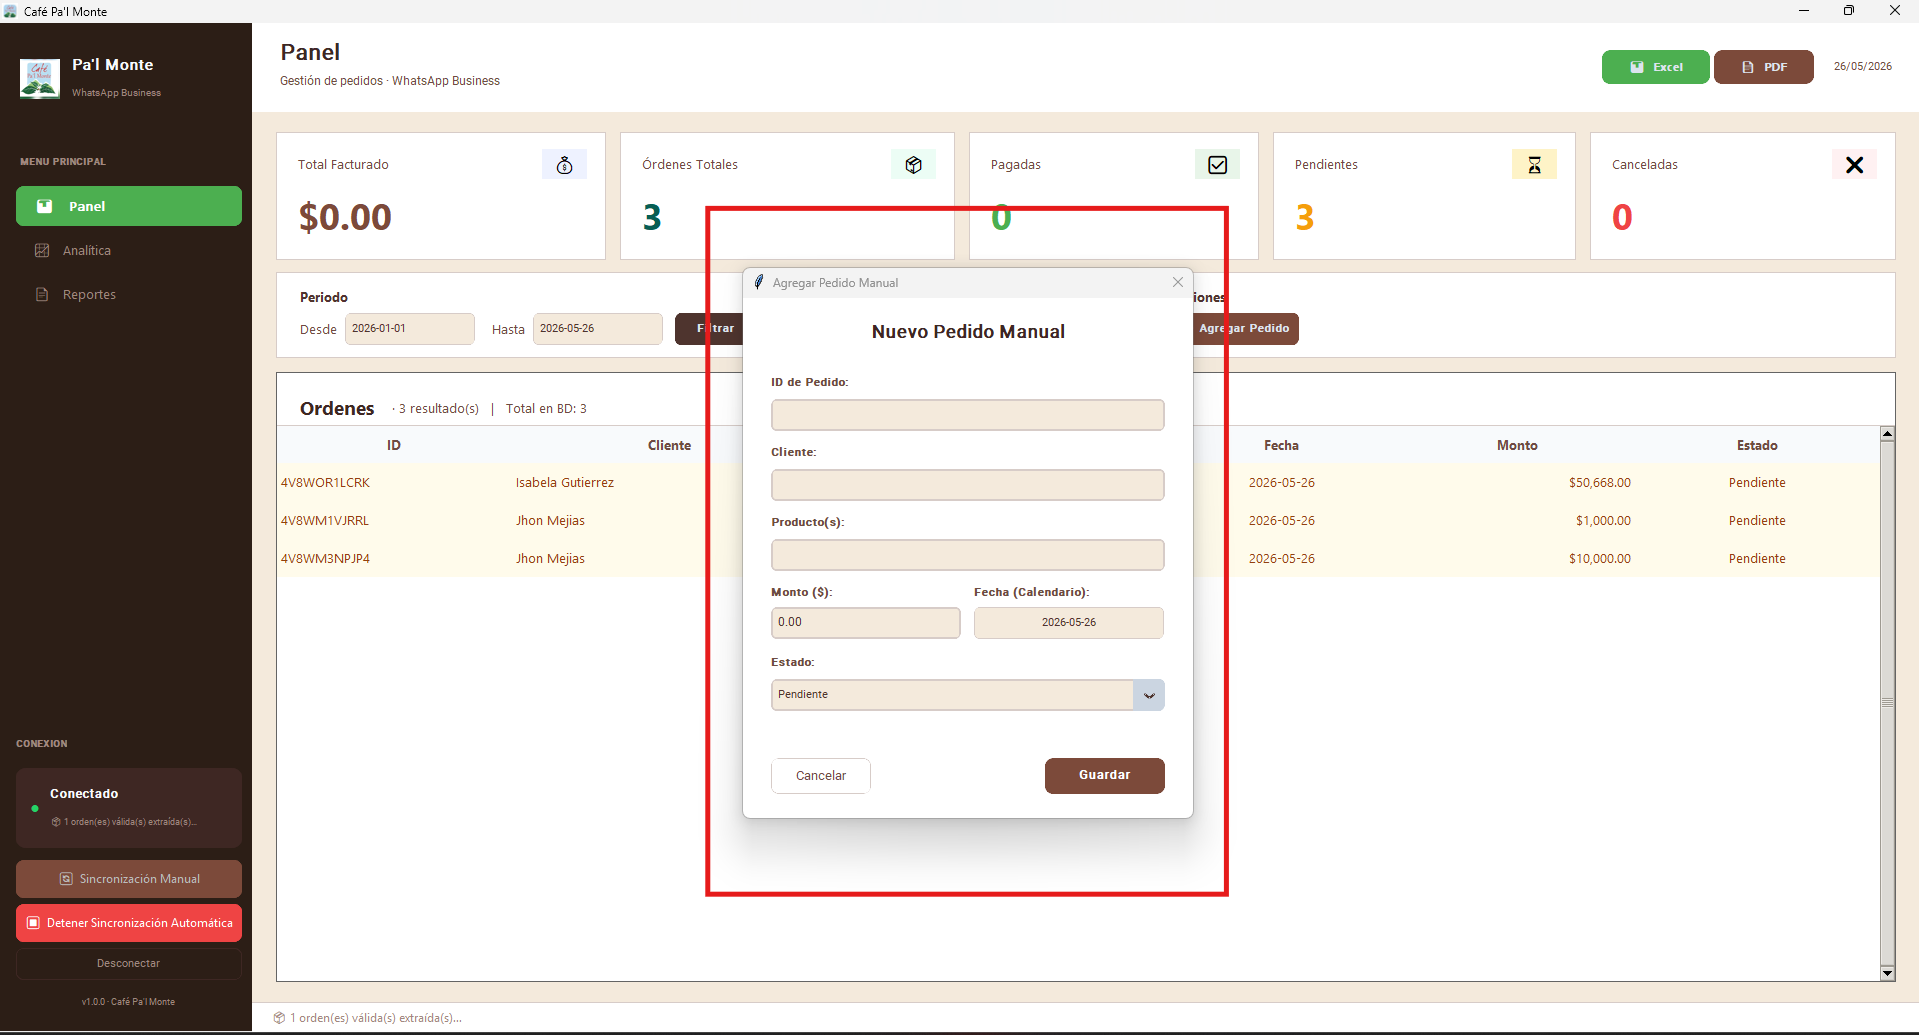
\includegraphics[width=0.55\textwidth]{image7.png}
    \caption{Formulario para el registro manual de un pedido.}
    \label{fig:add_form}
\end{figure}

\begin{enumerate}
    \setcounter{enumi}{2}
    \item Complete los siguientes campos obligatorios:
    \begin{itemize}
        \item \textbf{ID del Pedido:} Ingrese un código único identificador (pueden ser caracteres alfanuméricos).
        \item \textbf{Cliente:} Nombre completo o contacto del comprador.
        \item \textbf{Producto/Detalle:} Descripción corta del producto adquirido.
        \item \textbf{Fecha:} Fecha de realización de la compra (por defecto muestra el día actual).
        \item \textbf{Monto:} Valor total del pedido.
        \item \textbf{Estado:} Seleccione una categoría (Completado, Pendiente, Cancelado, Enviado, Envío en preparación, Entregado).
    \end{itemize}
    \item Presione \textbf{Guardar}. El pedido se agregará a la base de datos y se listará de inmediato en el Panel.
\end{enumerate}

\subsection{Acciones y Menú Contextual de la Tabla}
La tabla central contiene la lista de pedidos del periodo seleccionado. El sistema permite realizar modificaciones rápidas sobre cualquier pedido existente en la base de datos a través de clics en la fila respectiva:

\begin{figure}[H]
    \centering
    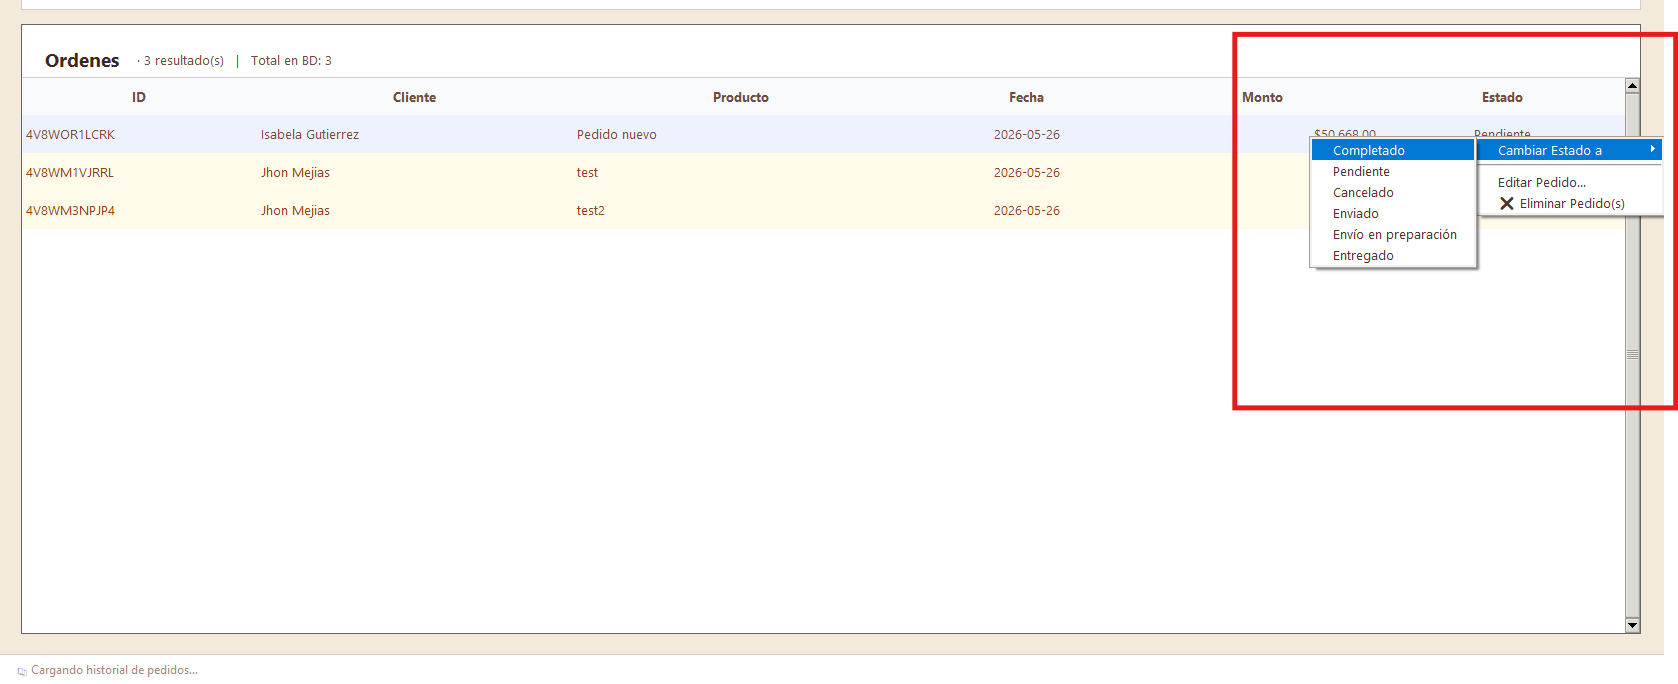
\includegraphics[width=0.7\textwidth]{image8.png}
    \caption{Menú contextual al hacer clic derecho sobre una orden de la lista.}
    \label{fig:context_menu}
\end{figure}

\begin{itemize}
    \item \textbf{Clic Derecho (Menú contextual):} Al hacer clic derecho sobre cualquier fila de la tabla de pedidos, aparecerá un menú flotante con las siguientes opciones directas:
    \begin{itemize}
        \item \textbf{Editar Pedido:} Abre un formulario idéntico al de creación manual con los datos actuales precargados para realizar correcciones ortográficas o de valor.
        \item \textbf{Cambiar Estado:} Permite alternar rápidamente el estado del pedido entre Completado, Enviado, Envío en preparación, Entregado, Pendiente o Cancelado sin necesidad de abrir la ventana de edición.
        \item \textbf{Eliminar Pedido:} Elimina definitivamente el pedido de la base de datos local.
    \end{itemize}
    \item \textbf{Doble Clic:} Al dar doble clic izquierdo continuo sobre una fila, el sistema abrirá de manera directa la ventana de \textbf{Edición de Pedido} para facilitar su edición.
\end{itemize}

\newpage

% ==========================================
% ANALÍTICA
% ==========================================
\section{Módulo de Analítica y Estadísticas}

El módulo de \textbf{Analítica} proporciona información comercial valiosa a partir de la acumulación histórica de pedidos. Este módulo traduce los números de la base de datos en información visual interactiva estructurada para fines de planeación del negocio.

\subsection{Filtros de Análisis}
En la parte superior de la pestaña se encuentra la barra de delimitación de datos de analítica. El usuario puede seleccionar un año y un mes específicos, o elegir \textbf{``Todos''} del menú de meses para analizar la operación histórica anual agregada de forma inmediata.

\begin{figure}[H]
    \centering
    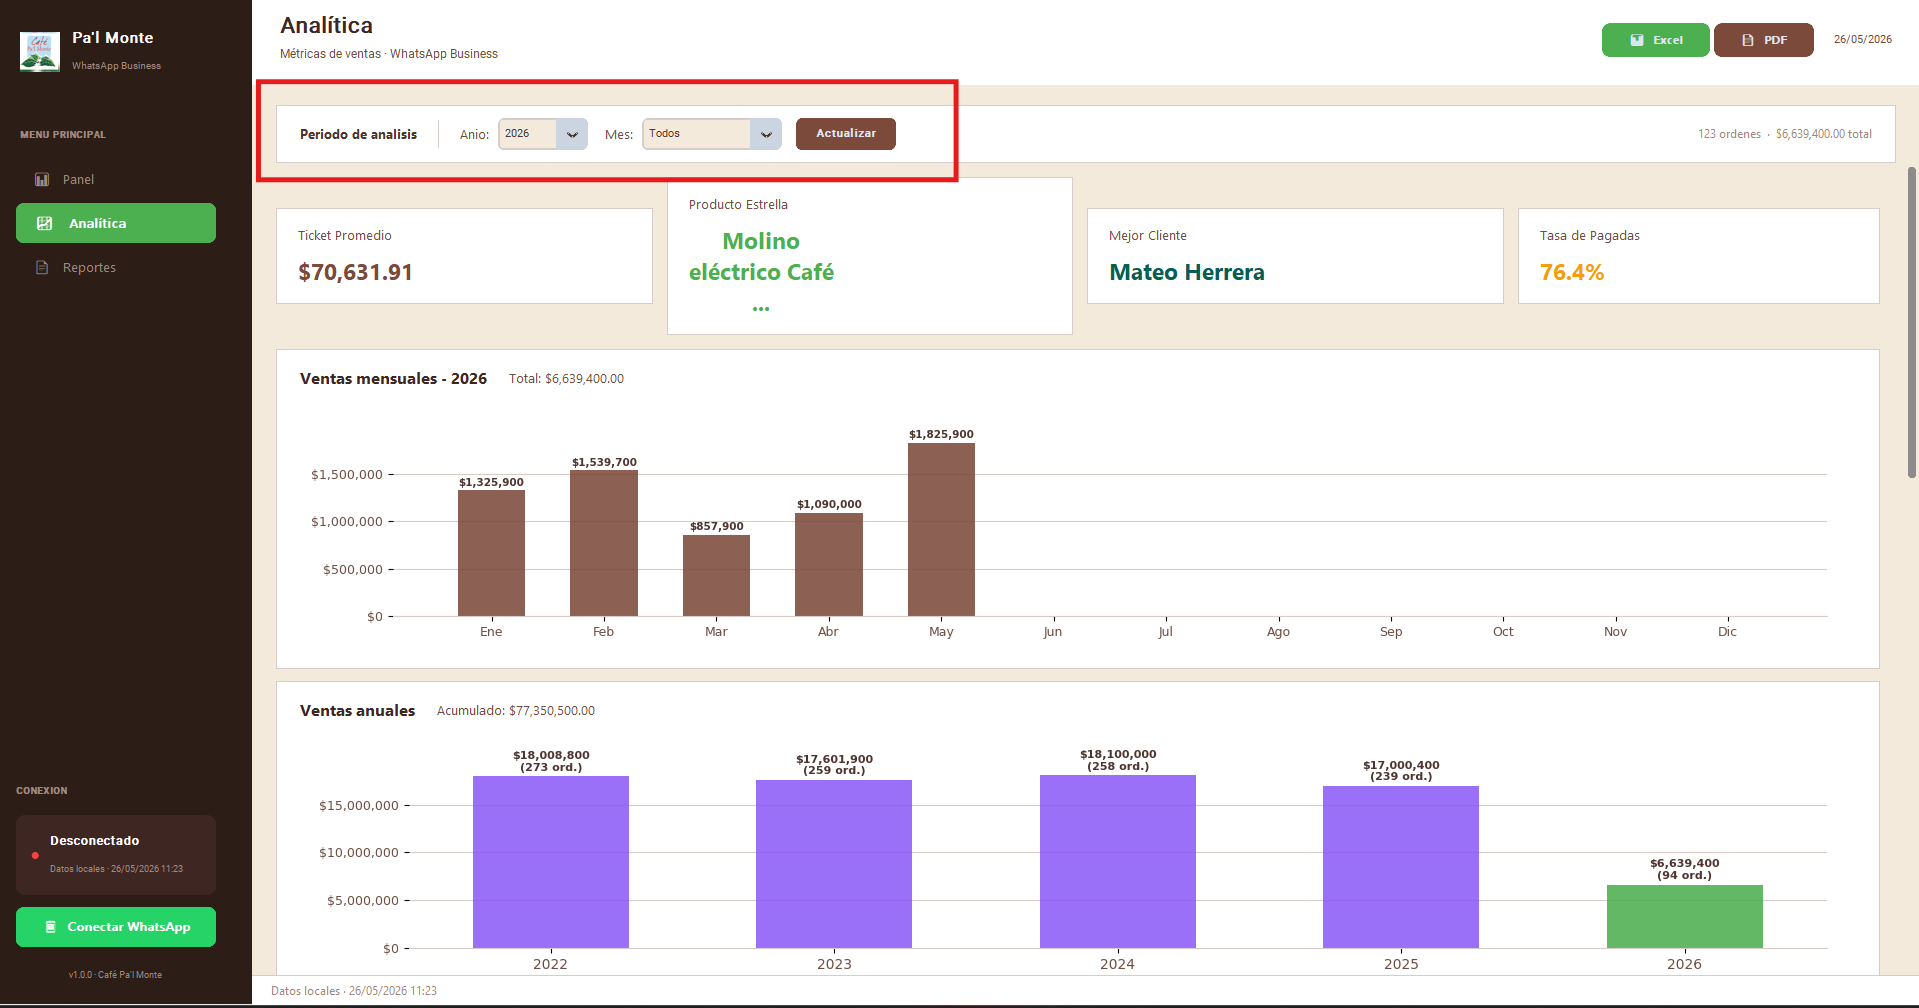
\includegraphics[width=0.9\textwidth]{image12.png}
    \caption{Controles de periodo y botón para actualizar gráficos.}
    \label{fig:an_filter}
\end{figure}

Al ajustar las variables de año y mes, presione el botón \textbf{``Actualizar''} para recalcular los gráficos inferiores y refrescar las tarjetas de analítica.

\subsection{KPIs de Gestión Analítica}
Esta sección provee métricas deducidas calculadas de forma inteligente para el periodo establecido:
\begin{itemize}
    \item \textbf{Ticket Promedio:} El gasto medio realizado por pedido (Ingresos Totales divididos entre el número de órdenes válidas pagadas).
    \item \textbf{Producto Estrella:} Aquel artículo o descripción de producto que ha generado el mayor volumen de facturación en el rango consultado.
    \item \textbf{Mejor Cliente:} El comprador que registra la mayor cantidad acumulada de aportación financiera al negocio.
    \item \textbf{Tasa de Pagadas:} Porcentaje de órdenes que se consolidaron con éxito sobre el total de registros en el sistema (tasa de conversión comercial).
\end{itemize}

\subsection{Gráficos de la Operación}
El sistema dibuja en pantalla múltiples paneles gráficos adaptativos:

\begin{figure}[H]
    \centering
    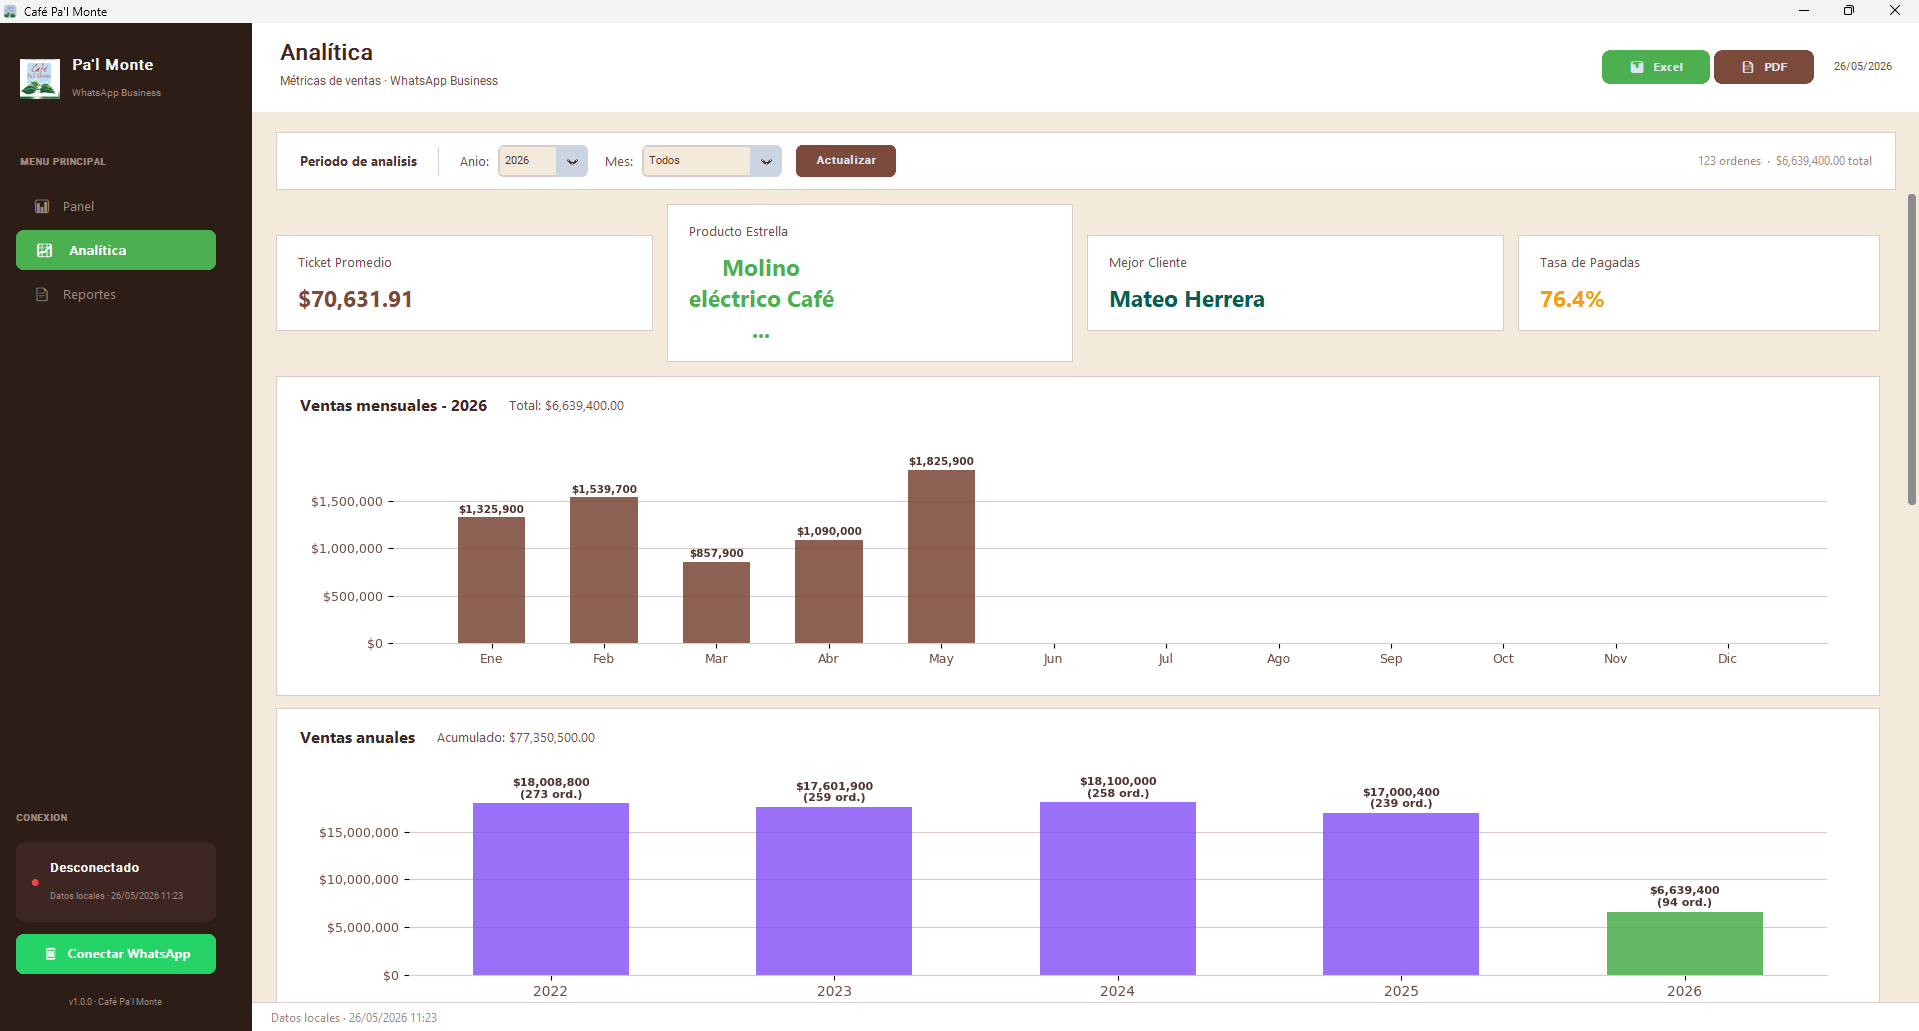
\includegraphics[width=0.85\textwidth]{image9.png}
    \caption{Gráficos de ventas mensuales y comparativa de facturación anual.}
    \label{fig:chart_sales}
\end{figure}

\begin{figure}[H]
    \centering
    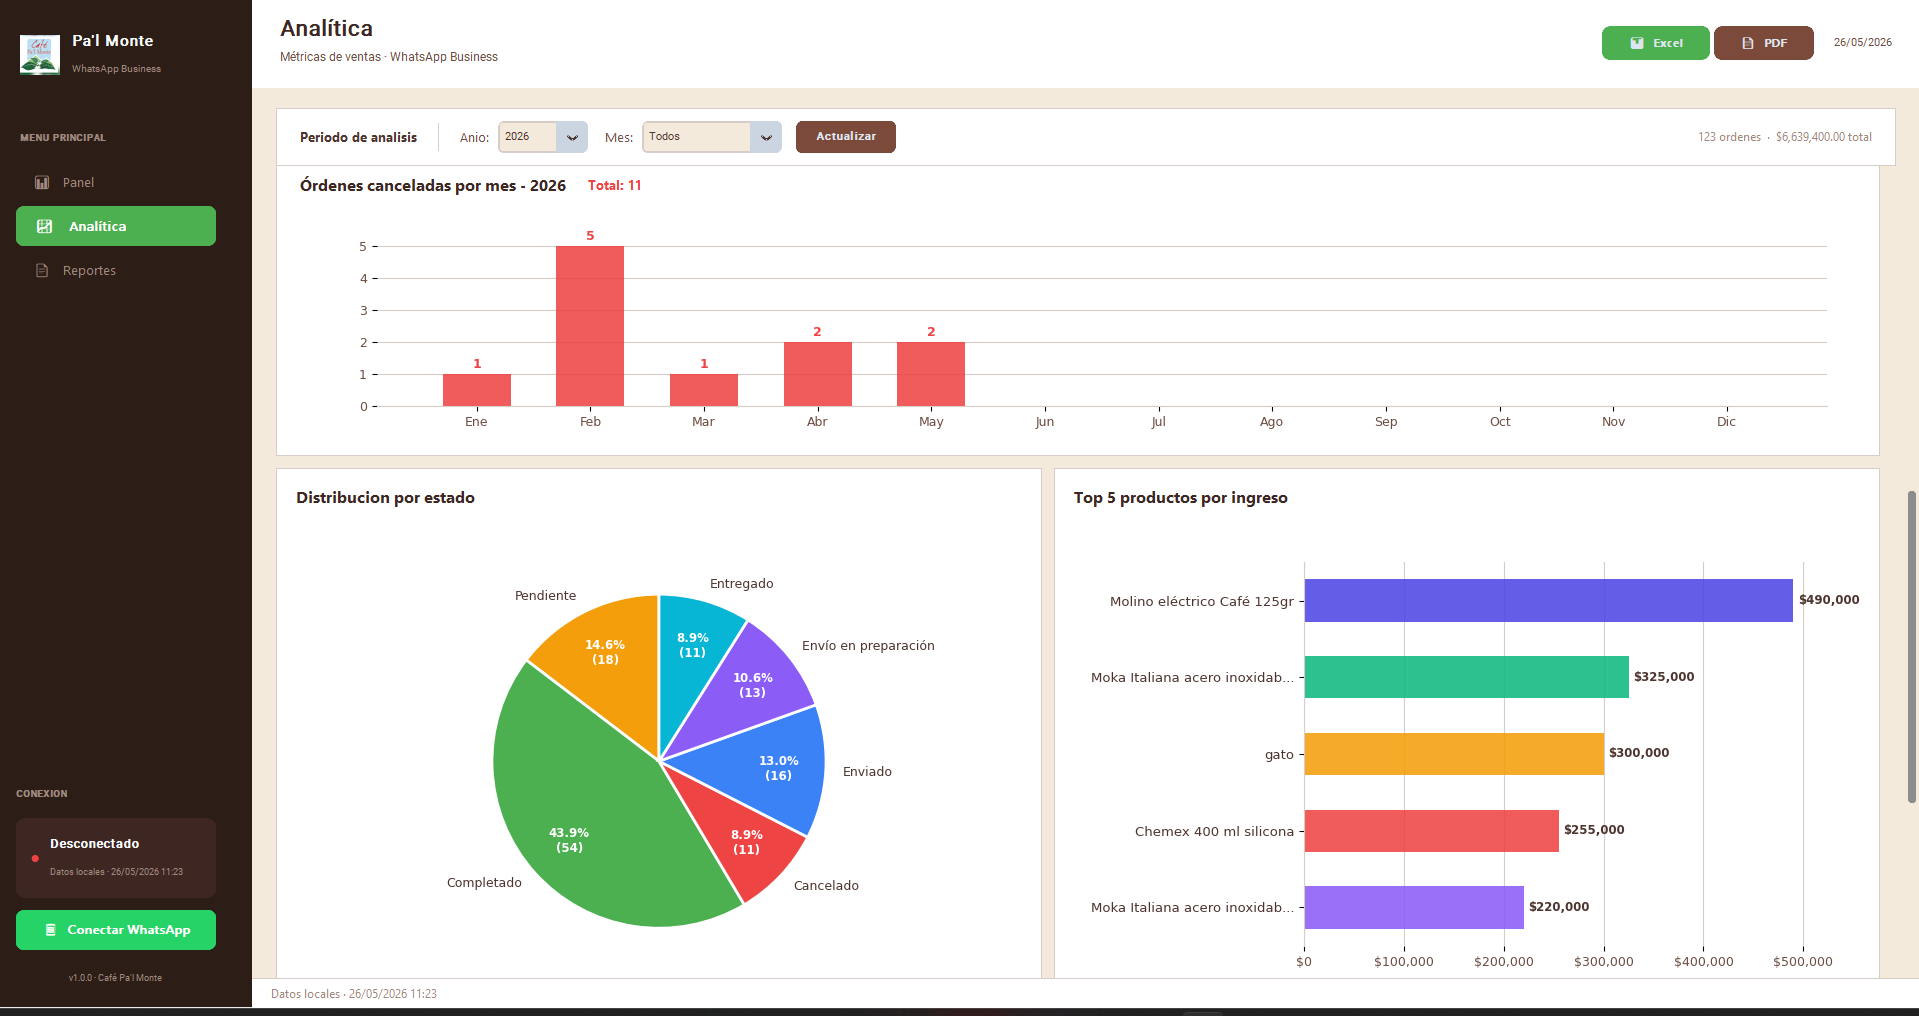
\includegraphics[width=0.85\textwidth]{image10.png}
    \caption{Histórico mensual de órdenes canceladas.}
    \label{fig:chart_cancelled}
\end{figure}

\begin{figure}[H]
    \centering
    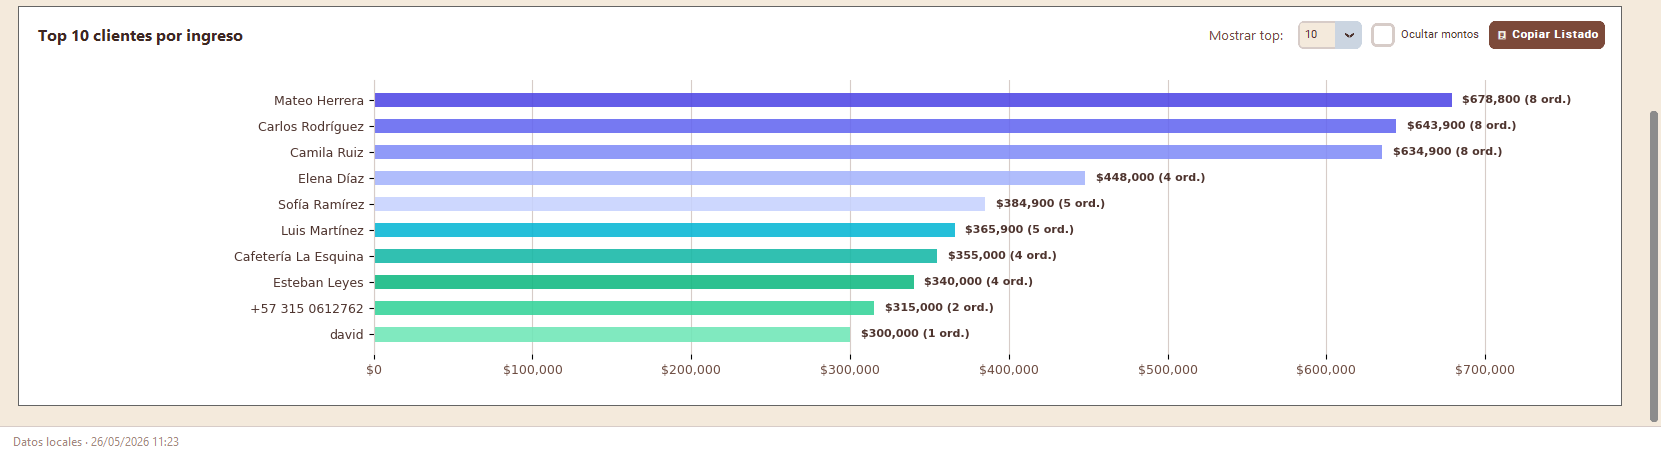
\includegraphics[width=0.85\textwidth]{image11.png}
    \caption{Distribución porcentual por estados de entrega y top de productos más vendidos.}
    \label{fig:chart_distribution}
\end{figure}

\begin{itemize}
    \item \textbf{Ventas Mensuales (Línea / Barra):} Comportamiento temporal del volumen facturado a lo largo del año consultado, mes a mes.
    \item \textbf{Ventas Anuales (Comparativo):} Permite superponer el rendimiento de facturación del año en curso contra periodos anteriores para analizar el crecimiento interanual.
    \item \textbf{Órdenes Canceladas por Mes:} Gráfico que reporta anomalías operativas o clientes que cancelaron compras recurrentemente por mes.
    \item \textbf{Distribución por Estado (Gráfico de Pastel):} Refleja de forma visual el porcentaje de órdenes que concluyen en entrega exitosa contra las que quedan suspendidas o devueltas.
    \item \textbf{Top 5 Productos:} Ranking vertical de artículos que reportan mayor entrada de dinero para el negocio.
    \item \textbf{Top de Clientes:} Lista ordenada de los contactos más leales por su volumen total acumulado de compra.
\end{itemize}

\newpage

% ==========================================
% EXPORTACIÓN Y REPORTES
% ==========================================
\section{Módulo de Reportes y Exportación}

La consolidación y entrega de información a departamentos de contabilidad o socios del negocio se realiza a través de las opciones de exportación del software.

\subsection{Botones de Exportación Rápida}
En la esquina superior derecha de la barra superior general del programa (visible desde cualquier pestaña), se localizan de manera permanente dos botones de exportación rápida:

\begin{figure}[H]
    \centering
    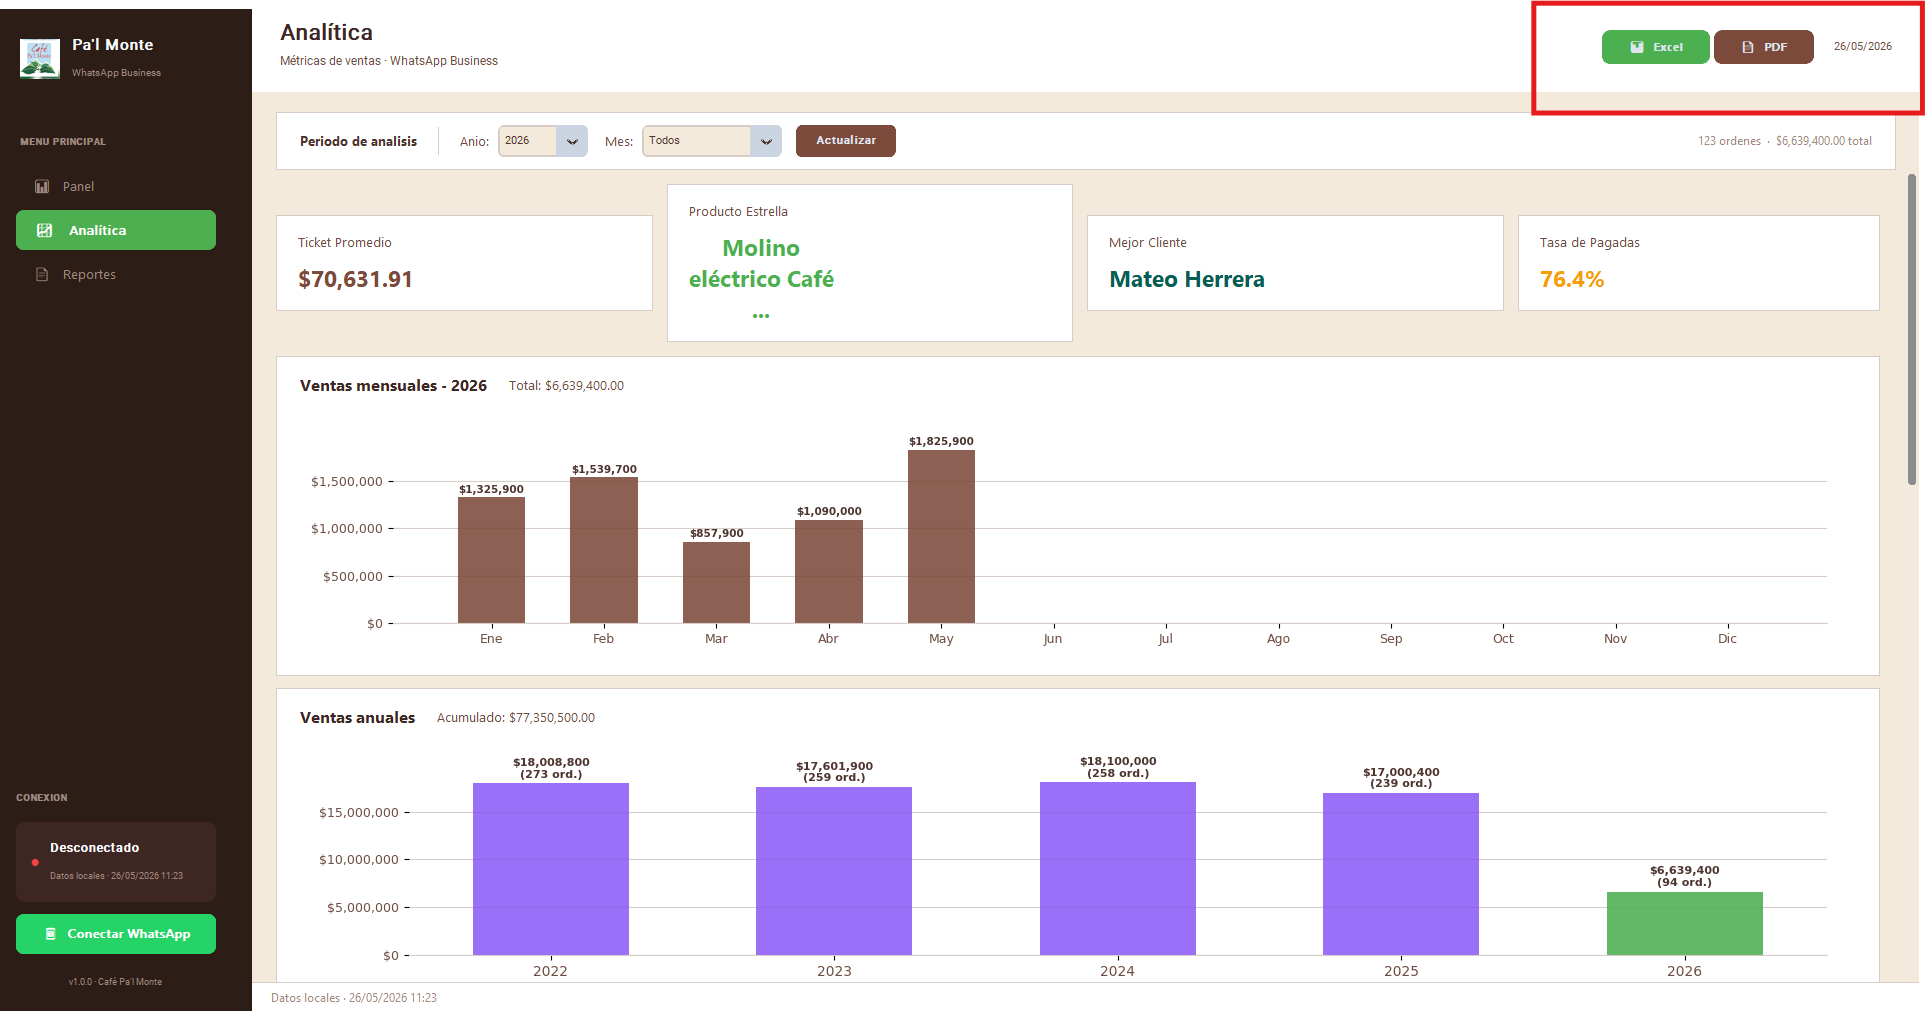
\includegraphics[width=0.45\textwidth]{image13.png}
    \caption{Botones de exportación rápida en formato PDF y Excel.}
    \label{fig:export_buttons}
\end{figure}

\begin{itemize}
    \item \textbf{Botón PDF (icono de hoja con texto):} Exporta la información que esté actualmente filtrada en el Panel a un reporte formateado en PDF de diseño corporativo.
    \item \textbf{Botón Excel (icono de gráfico de barras):} Genera un libro de cálculo contable enriquecido.
\end{itemize}

Al ser presionados, el sistema emite el archivo correspondiente en la carpeta del sistema y lo abre de manera automática usando el visor nativo de su computadora (su lector de PDF predeterminado o Microsoft Excel, respectivamente).

\subsection{Pestaña de Historial de Reportes}
El módulo dedicado de \textbf{Reportes} del menú lateral organiza el almacenamiento y permite la creación estructurada de reportes en periodos tradicionales:

\begin{figure}[H]
    \centering
    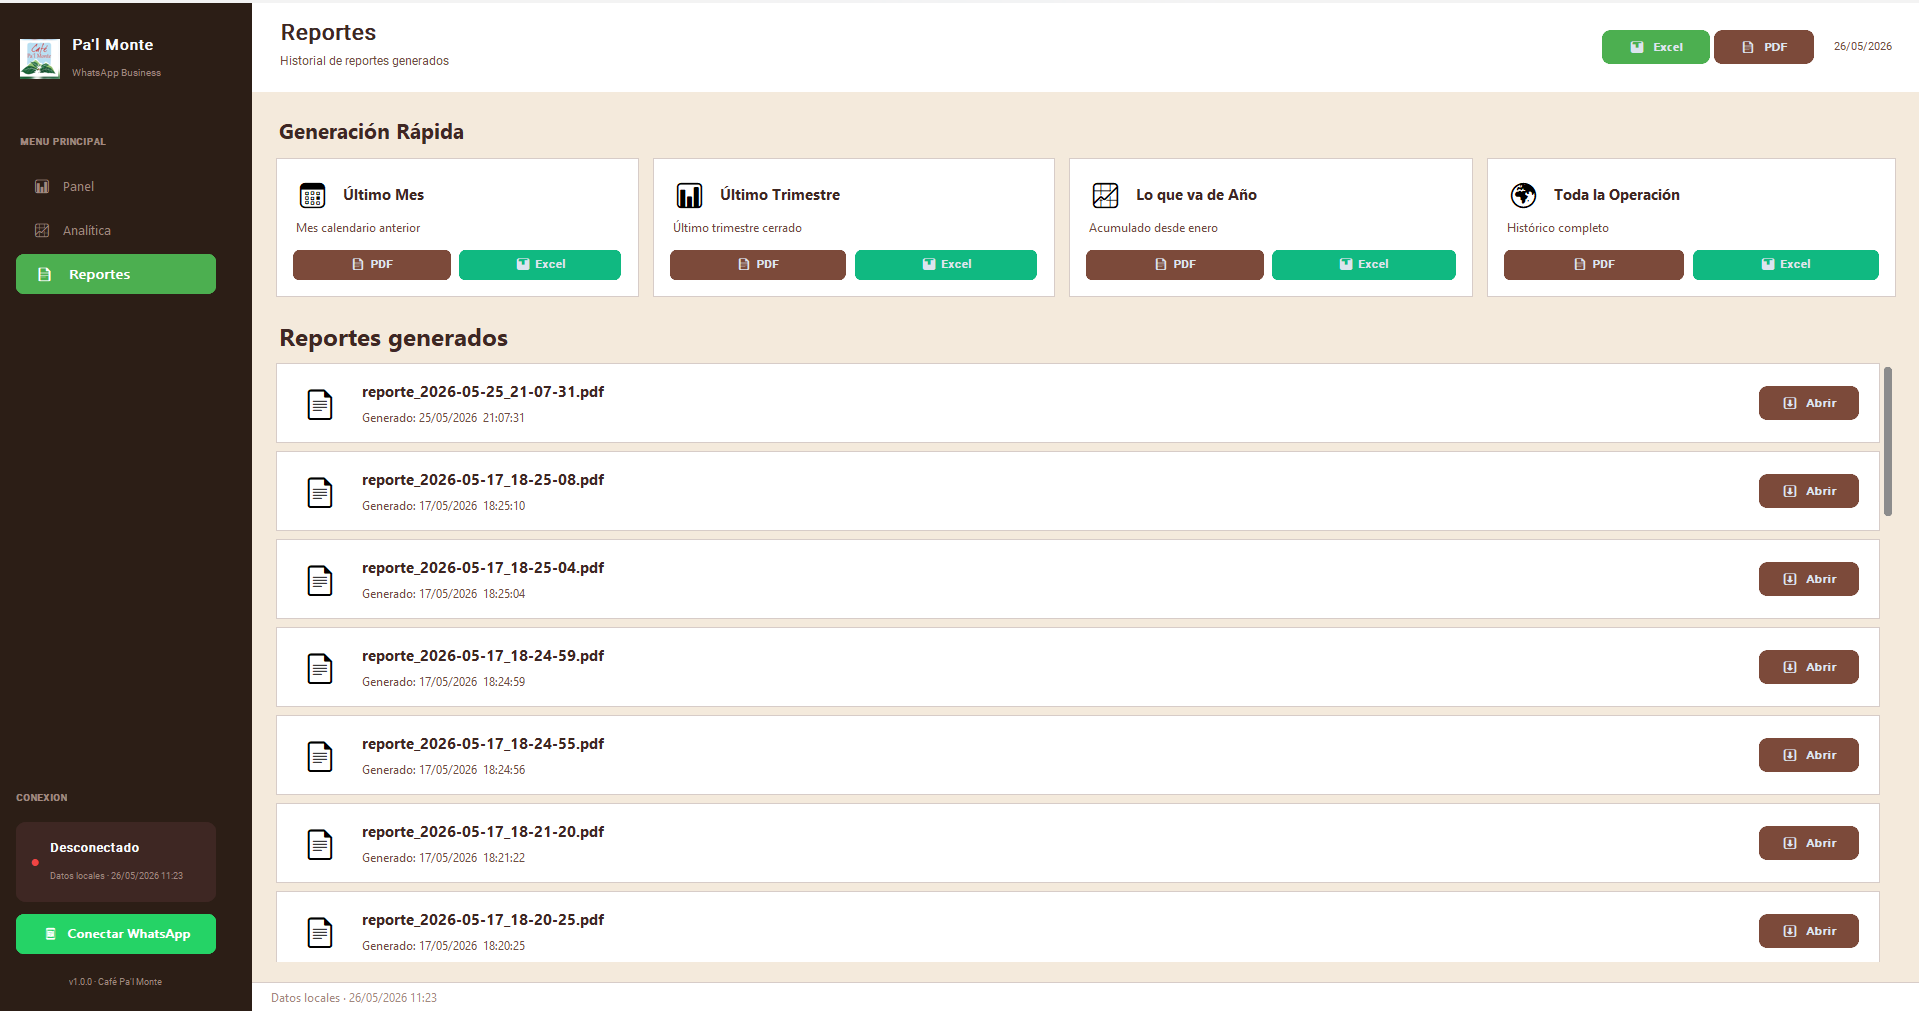
\includegraphics[width=0.9\textwidth]{image14.png}
    \caption{Vista general del Módulo de Reportes con opciones rápidas e historial de archivos.}
    \label{fig:reports_overview}
\end{figure}

\begin{itemize}
    \item \textbf{Sección de Generación Rápida:} Botones automatizados para procesar información sin necesidad de ajustar filtros manuales. Los rangos integrados son:
    \begin{itemize}
        \item \textbf{Último Mes:} Facturación correspondiente a los últimos 30 días calendario.
        \item \textbf{Último Trimestre:} Información comercial de los últimos 90 días transcurridos.
        \item \textbf{Lo que va del Año:} Consolidado comercial desde el primero de enero del año vigente hasta la fecha.
        \item \textbf{Toda la Operación:} Exportación total de la base de datos local desde la primera fecha de registro guardada.
    \end{itemize}
    \item \textbf{Historial de Reportes Generados:} Tabla inferior que registra de forma detallada todos los reportes generados a lo largo del uso de la aplicación. Muestra el nombre del archivo, tipo de formato y proporciona un botón directo de \textbf{``Abrir''} para acceder al reporte físico sin necesidad de buscarlo manualmente en el explorador de archivos de Windows.
\end{itemize}

\subsection{Formato de los Reportes Generados}
Los archivos exportados son estructurados con fines administrativos:
\begin{itemize}
    \item \textbf{Reporte PDF:} Diseñado para impresión directa. Contiene membrete formal, cabecera de KPIs del periodo con fondo corporativo de la marca Café Pa'l Monte, una tabla formateada con filas alternadas (cebra), celdas de estado destacadas por colores semáforo para rápida lectura visual, y totalización al final del documento.
    \item \textbf{Hoja de Cálculo Excel:} Diseñada para contabilidad avanzada. Muestra la lista de órdenes procesada en una pestaña primaria con celdas numéricas formateadas financieramente y totalización integrada. Posee una segunda pestaña de ``Resumen'' que expone las métricas clave e incorpora de forma automática un gráfico de columnas en 3D que mapea la cantidad de órdenes según su estado de entrega.
\end{itemize}

\newpage

% ==========================================
% RESOLUCIÓN DE PROBLEMAS
% ==========================================
\section{Solución a Problemas Frecuentes (FAQ)}

En el uso diario del software pueden ocurrir desconexiones o bloqueos causados por interrupciones de red o actualizaciones de servicios externos de WhatsApp. A continuación se presentan las soluciones recomendadas ante estas contingencias.

\subsection{Problema de Vinculación de WhatsApp o Pantalla Congelada}
\textbf{Síntoma:} Al hacer clic en ``Conectar WhatsApp'', la ventana del navegador no carga el código QR, se queda en blanco o muestra un aviso de error continuo. O bien, el teléfono reporta que la sesión está activa pero el panel del programa sigue indicando ``Desconectado''.\\
\textbf{Solución:}
\begin{enumerate}
    \item Cierre la ventana del navegador controlado si continúa abierta.
    \item Cierre la aplicación \textbf{Café Pa'l Monte Gestión}.
    \item Abra la carpeta del programa donde se encuentra el ejecutable y localice una carpeta llamada \textbf{wsp\_session\_edge} (o similar). Esta carpeta almacena los datos de inicio de sesión de la sesión controlada.
    \item Haga clic derecho sobre la carpeta \textbf{wsp\_session\_edge} y seleccione la opción \textbf{Eliminar}.
    \item Inicie la aplicación nuevamente y haga clic en \textbf{``Conectar WhatsApp''}. La sesión se habrá limpiado por completo y le solicitará de inmediato escanear un nuevo código QR.
\end{enumerate}

\subsection{El Navegador no se Abre al Presionar ``Conectar WhatsApp''}
\textbf{Síntoma:} Al presionar el botón verde de conexión, no se despliega ninguna ventana del navegador controlado en la computadora.\\
\textbf{Solución:}
\begin{itemize}
    \item Verifique que tiene instalado en su computadora \textbf{Microsoft Edge} o \textbf{Google Chrome} en su versión estándar para Windows.
    \item Compruebe que su antivirus o el Firewall de Windows Defender no estén bloqueando la automatización de la aplicación. Si le aparece una advertencia del sistema la primera vez, asegúrese de hacer clic en \textbf{``Permitir acceso''}.
\end{itemize}

\subsection{Los Pedidos Recibidos no Aparecen en la Tabla}
\textbf{Síntoma:} Un cliente realizó una orden por WhatsApp Business pero esta no se carga en la tabla del panel del programa, a pesar de estar conectado.\\
\textbf{Solución:}
\begin{enumerate}
    \item Asegúrese de que el pedido haya sido registrado de manera formal en el menú de \textbf{``Pedidos''} dentro del chat correspondiente en su aplicación de WhatsApp Business en el celular. El sistema lee únicamente las órdenes creadas formalmente a través de la herramienta de Pedidos de WhatsApp Business, no de mensajes de texto sueltos del chat.
    \item Compruebe que su celular tenga conexión a internet activa y no se encuentre en modo de ahorro de energía agresivo.
    \item Presione el botón de \textbf{``Sincronización Manual''} en el panel izquierdo de la aplicación para forzar al navegador a revisar los chats de pedidos en ese instante.
\end{enumerate}

\subsection{El Total Facturado es Menor al Esperado}
\textbf{Síntoma:} La sumétrica de ingresos acumulada en el Panel es menor a la que se calcula manualmente sumando todas las órdenes del periodo.\\
\textbf{Solución:}
\begin{itemize}
    \item Recuerde que el sistema aplica reglas de cálculo financiero formal: \textbf{excluye del total facturado las órdenes cuyo estado sea ``Pendiente'' o ``Cancelado''}. Únicamente se integran a los ingresos las órdenes bajo estados de cobro efectivo (Completado, Enviado, Envío en preparación y Entregado). Verifique si hay órdenes pendientes de cobro que alteren su suma manual.
\end{itemize}

\subsection{Copia de Seguridad de la Información}
\textbf{Síntoma:} Desea formatear la computadora o migrar el sistema a otro equipo y no quiere perder el histórico de pedidos acumulado de forma local.\\
\textbf{Solución:}
\begin{itemize}
    \item Toda la información de pedidos, reportes e historial manual se almacena localmente en la carpeta del programa. Localice el archivo llamado \textbf{orders.db} dentro de la subcarpeta de ejecución.
    \item Realice una copia periódica de este archivo en un disco externo o servicio de almacenamiento en la nube. Al migrar la aplicación a otra máquina, simplemente pegue su archivo \textbf{orders.db} respaldado en el mismo directorio de la aplicación antes de iniciarla por primera vez y recuperará todas sus transacciones.
\end{itemize}

\end{document}
